\documentclass[a4paper,12pt]{report}
\usepackage{makecell}
\usepackage{placeins}
\usepackage[T5]{fontenc}
\usepackage[american]{babel}
\usepackage[margin=1in]{geometry}
\usepackage{tikz}
\usepackage{amssymb}
\usetikzlibrary{calc}
\usepackage{graphicx}
\usepackage{lmodern}
\usepackage{titlesec}
\titlespacing*{\chapter}{0pt}{0pt}{0pt}
\usepackage{fancyhdr}
\pagestyle{fancy}
\setlength{\headheight}{15pt}
\addtolength{\topmargin}{-2.5pt}
\fancyhead[L]{}
\fancyhead[R]{\textit{\MakeUppercase{\leftmark}}}
\usepackage{amsmath}
\usepackage{array, booktabs, multirow, longtable}
\usepackage{tabularx}
\usepackage{adjustbox}
\usepackage{newunicodechar}
\newunicodechar{≈}{\approx}
\usepackage{listings}
\usepackage{caption}
\usepackage{subcaption}
\usepackage{float}
\usepackage{tocloft}
\usepackage[colorlinks=true, linkcolor=black, citecolor=black, urlcolor=black]{hyperref}
\usepackage{bookmark}
\usepackage{lipsum}
\usepackage{cite}
\usepackage{setspace}
\definecolor{codegreen}{rgb}{0,0.6,0}
\definecolor{codegray}{rgb}{0.5,0.5,0.5}
\definecolor{codepurple}{rgb}{0.58,0,0.82}
\definecolor{backcolour}{rgb}{0.95,0.95,0.92}
\lstdefinestyle{mystyle}{
    backgroundcolor=\color{backcolour},
    commentstyle=\color{codegreen},
    keywordstyle=\color{magenta},
    numberstyle=\tiny\color{codegray},
    stringstyle=\color{codepurple},
    basicstyle=\ttfamily\footnotesize,
    breakatwhitespace=false,
    breaklines=true,
    captionpos=b,
    keepspaces=true,
    numbers=left,
    numbersep=5pt,
    showlines=false,
    showspaces=false,
    showstringspaces=false,
    showtabs=false,
    tabsize=2
}
\lstset{style=mystyle, showlines=false}
% Glossaries are not used in this document, so disable the package to avoid warnings.
% \usepackage[acronym]{glossaries}
% \makeglossaries

\begin{document}

% ===== COVER PAGE =====

\thispagestyle{empty}
\begin{tikzpicture}[remember picture, overlay]
    \draw[line width=2pt]
        ($(current page.north east) - (0.5in, 0.5in)$);
\end{tikzpicture}
\begin{center}
    \adjustbox{max width=\textwidth}{\small \textbf{DEPARTMENT OF INFORMATION AND COMMUNICATION TECHNOLOGY}}\\[2cm]
    
\includegraphics[width=0.7\textwidth]{images/vast.png}\\[1.7cm]
    {\Huge \textbf{Report}}\\[1cm]
    \rule{\textwidth}{0.75pt}\\[0.6cm]
    {\LARGE \textbf{Week 3 - Security fundamentals for LLM applications}}\\[0.4cm]
    \rule{\textwidth}{0.75pt}\\[1.2cm]
    {\Large \textbf{By Nguyen Huy Hai, Dang Trung Hieu}}
\end{center}
\vfill
\begin{center}
    % Supervisor above date
    %{\large \textbf{Supervisor: Hoang Do Thanh Tung}} \\ \vspace{0.8cm}
    \textit{Ha Noi, October 2026}
\end{center}

\newpage


% ===== FRONT MATTER =====
\newpage
\pagenumbering{arabic}
\setcounter{page}{1}
\setlength{\parindent}{0pt}
\setlength{\parskip}{3pt}

% \newpage
% \tableofcontents

% \newpage
% \listoffigures
% \addcontentsline{toc}{chapter}{List of Figures}

% \newpage
% \listoftables
% \addcontentsline{toc}{chapter}{List of Tables}

% \newpage
% \chapter*{List of Abbreviations}
% \addcontentsline{toc}{chapter}{List of Abbreviations}
% {
% \renewcommand{\arraystretch}{1.3}
% \begin{longtable}{@{}lp{12cm}@{}}
% \toprule
% Term & Definition \\ 
% \midrule
% WF   & Work Flow \\
% \bottomrule
% \end{longtable}
% }
% \markboth{List of Abbreviations}{}

\newpage
\chapter{Work in This Week}

\section{Assistant Architecture and Threat Modeling}
Map a simple assistant: user request → supporting document → model → response. Draw three examples where the same input is benign task data versus an instruction.

\section{Meeting with the Korean Research Team}


\textbf{Meeting Objectives}
\begin{itemize}
    \item Present a summary of the project's background, objectives,
    and work completed so far.

    \item Discuss a long-term research plan with the Korean team,
    using the generation of 500 seed cases as an initial target.

    \item Paper research sharing and discussion.
\end{itemize}

\textbf{Research Paper Sharing}
\begin{enumerate}
    \item \href{https://arxiv.org/pdf/2504.18369}{Threat Modeling for Large Language Model-Integrated Applications (ThreMoLIA)}
    \item \href{https://arxiv.org/pdf/2202.03286}{Red Teaming Language Models with Language Models}
    \item \href{https://arxiv.org/pdf/2402.04249}{HarmBench: A Standardized Evaluation Framework for Automated Red Teaming and Robust Refusal}
    \item \href{https://owasp.org/www-project-top-10-for-large-language-model-applications/}{OWASP Top 10 for Large Language Model Applications}
\end{enumerate}


\section{Division of Work}
\noindent
Hai: based on the simple map assistant, identify and complete the list of attacker-controlled
surfaces including user text, retrieved documents, image OCR.

\noindent
Hieu: complete the attack-surface diagram, Develop five examples illustrating potential threats
and attack scenarios


%%%%%
\chapter{Attack surface diagram}
\begin{figure}[H]
    \centering
    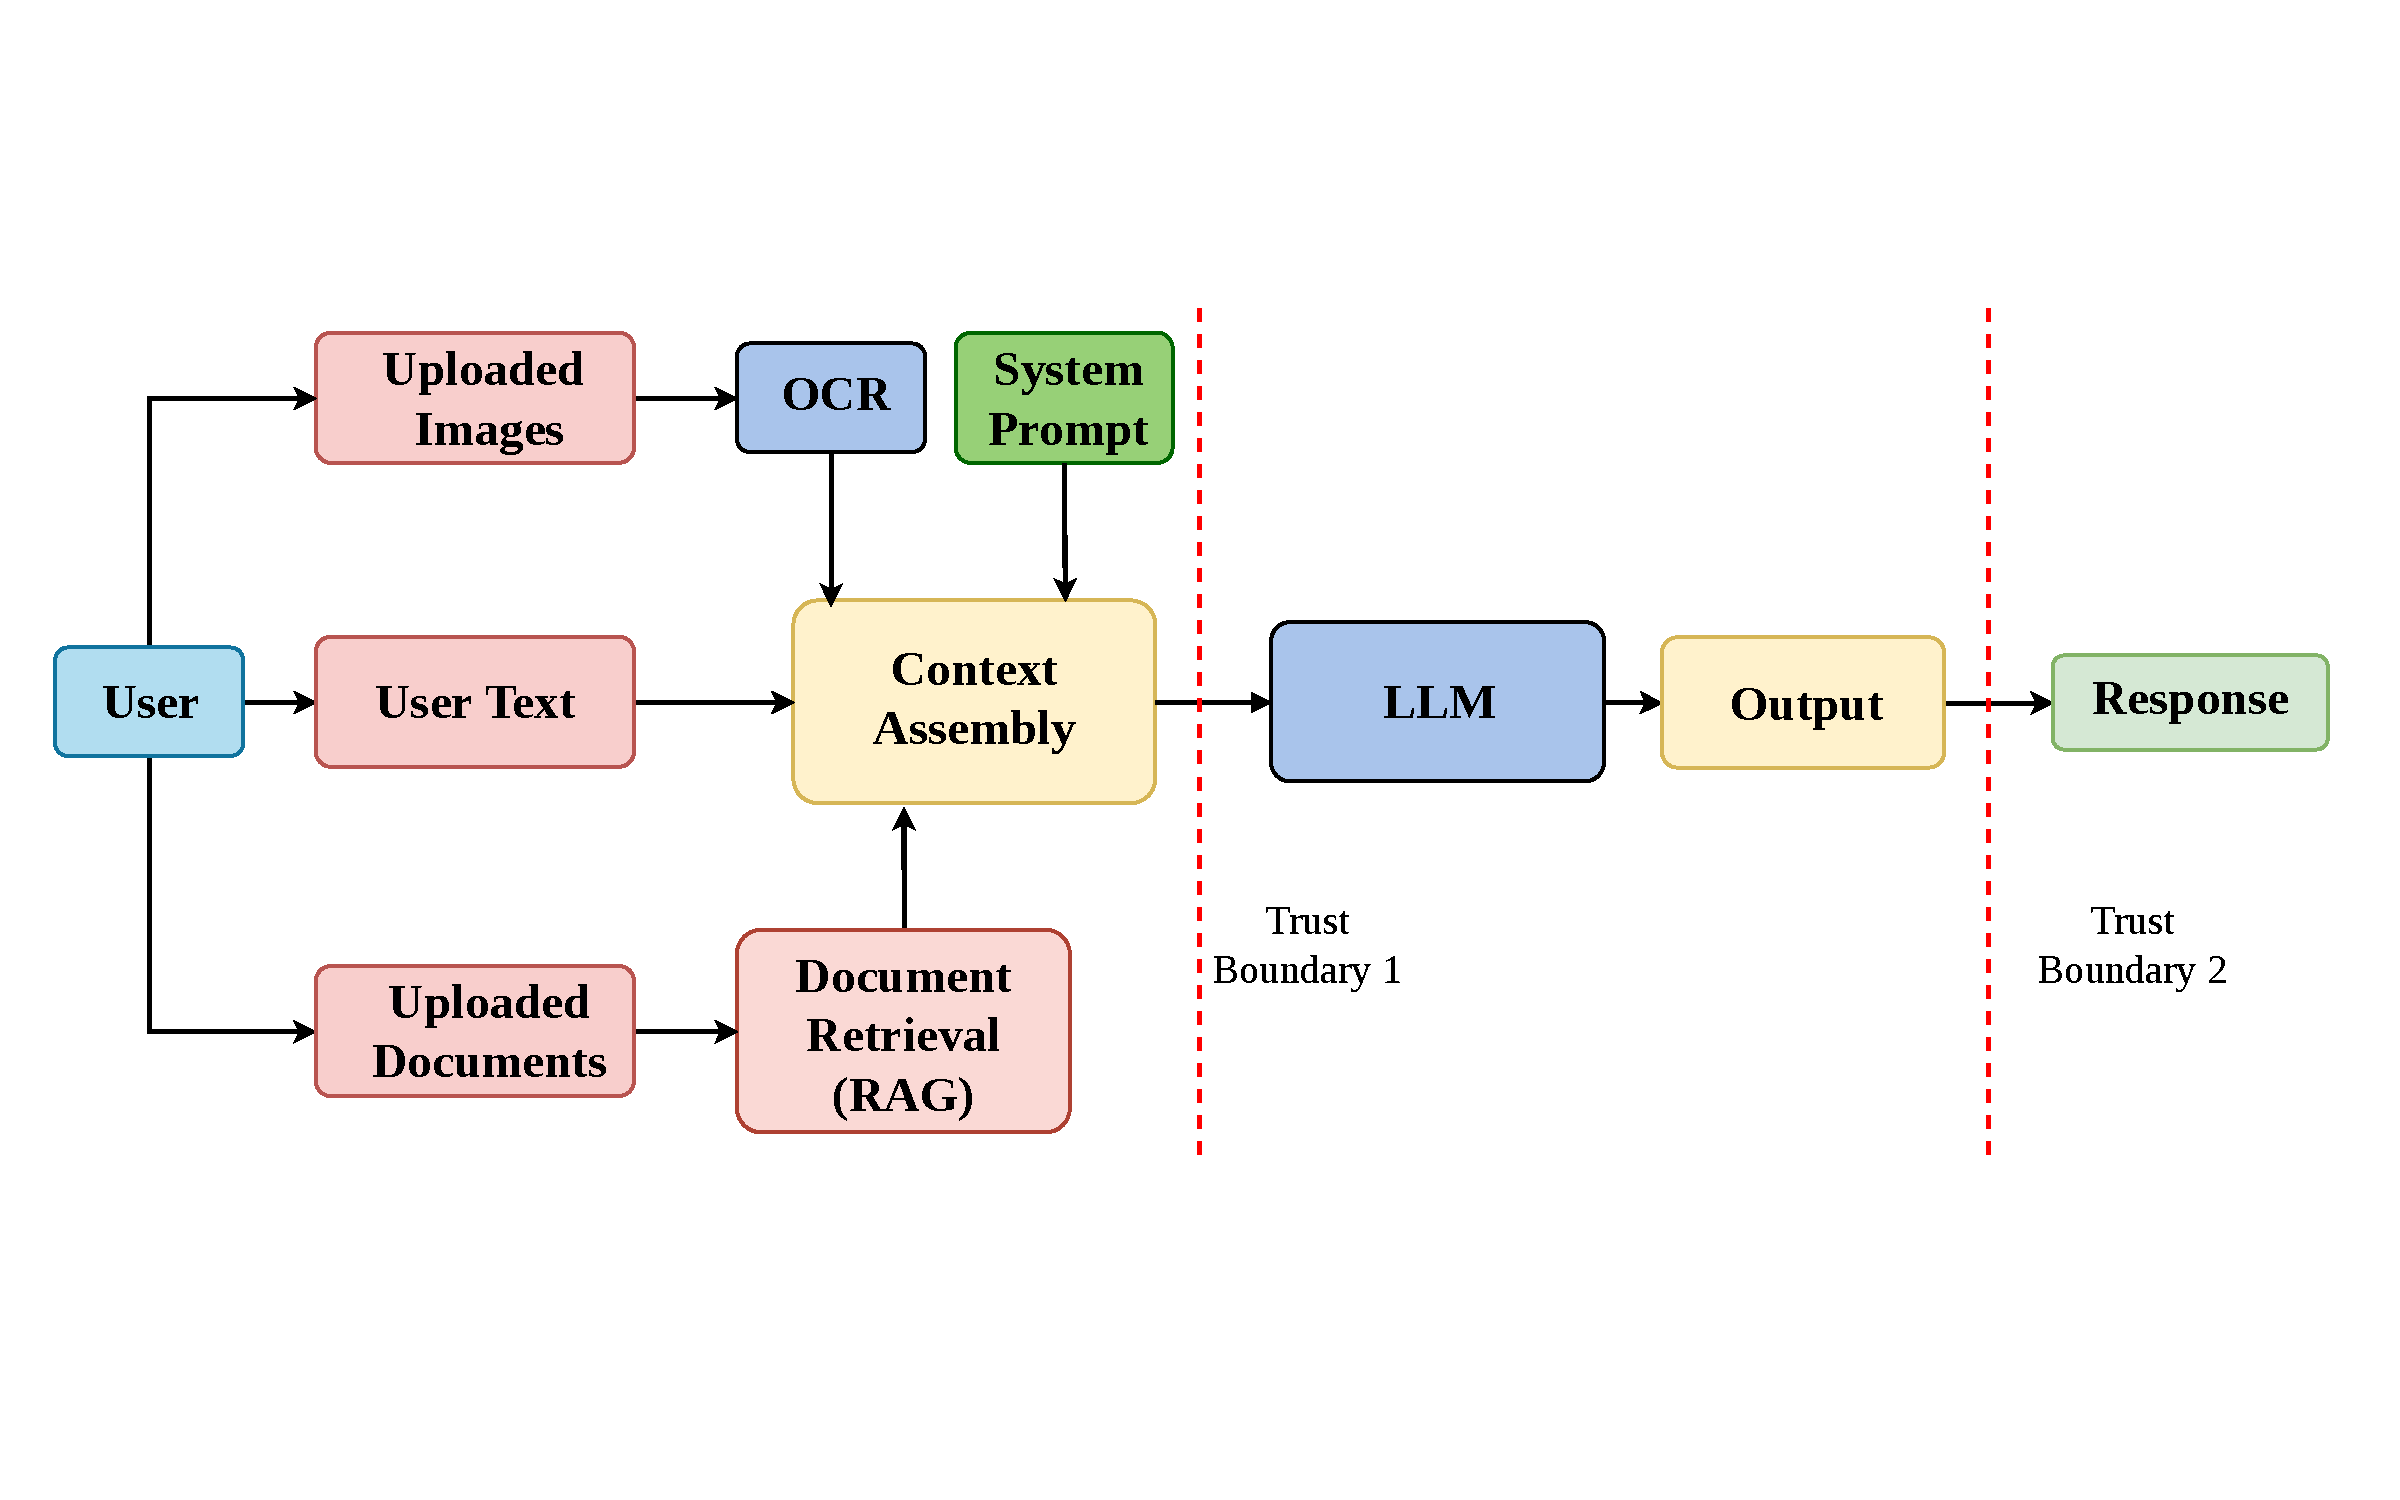
\includegraphics[width=1\textwidth]{images/Attack_surface_diagram.pdf}
    \caption{Architecture sketch}
    \label{fig:simple_assistant}
\end{figure}

\textbf{Trust Boundary 1: Input Validation}

The first trust boundary focuses on input validation before information
is passed to the LLM, include: 

\begin{itemize}
    \item \textbf{Exceed token:} Check when the input exceeds the
    allowed token limit.

    \item \textbf{Prompt injection:} Detect potentially malicious
    instructions in user requests or retrieved documents that may
    attempt to manipulate the LLM's behavior.

    \item \textbf{Retrieval authentication:} Verify the authenticity
    and authorization of retrieved information from internal
    documents, official websites, databases, and the Internet.
\end{itemize}

\textbf{Trust Boundary 2: Output Security Checks}

The second trust boundary focuses on validating the LLM's generated
output before it is returned to the user, include: 

\begin{itemize}
    \item \textbf{Sensitive data leakage:} Check whether the generated
    response exposes sensitive or confidential information.

    \item \textbf{Response violation:} Check whether the generated
    response violates the application's security requirements.

    \item \textbf{Factual grounding:} Verify whether the generated
    response is supported by the retrieved information and relevant
    context.
\end{itemize}


\chapter{Examples}
\label{chap:examples}
\begin{table}[H]
    \centering
    \small
    \renewcommand{\arraystretch}{1.3}
    \begin{tabularx}{\textwidth}{
        |>{\centering\arraybackslash}p{0.7cm}
        |>{\raggedright\arraybackslash}p{2.7cm}
        |X
        |>{\raggedright\arraybackslash}p{2.5cm}|
    }
        \hline
        \textbf{No} &
        \textbf{Attacker-controlled Surface} &
        \textbf{Threat Statement} &
        \textbf{Potential Impact} \\
        \hline

        1 &
        User Text &
        A malicious user submits a prompt injection attempting to override the assistant's intended instructions and manipulate its behavior. &
        Confidentiality, Integrity \\
        \hline

        2 &
        Retrieved Documents &
        An attacker embeds malicious instructions in a document that is later retrieved by RAG, potentially manipulating the LLM's response. &
        Confidentiality, Integrity \\
        \hline

        3 &
        Image OCR &
        An attacker uploads an image containing hidden or misleading instructions that OCR extracts and passes to the LLM. &
        Confidentiality, Integrity \\
        \hline

        4 &
        Retrieved Documents &
        An attacker introduces falsified policy documents into the knowledge base, causing the assistant to generate inaccurate policy summaries. &
        Integrity \\
        \hline

        5 &
        User Text &
        A malicious user attempts to extract system instructions or confidential internal information through carefully crafted requests. &
        Confidentiality \\
        \hline
    \end{tabularx}
    \caption{Examples of attacker-controlled surfaces and potential threats}
    \label{tab:attacker_surfaces}
\end{table}



\end{document}